\documentclass{article}

% if you need to pass options to natbib, use, e.g.:
%     \PassOptionsToPackage{numbers, compress}{natbib}
% before loading neurips_2018

% ready for submission
% \usepackage{neurips_2018}

% to compile a preprint version, e.g., for submission to arXiv, add add the
% [preprint] option:
%     \usepackage[preprint]{neurips_2018}

% to compile a camera-ready version, add the [final] option, e.g.:
% \usepackage[final]{neurips_2018}

% to avoid loading the natbib package, add option nonatbib:
%     \usepackage[nonatbib]{neurips_2018}

\usepackage[utf8]{inputenc} % allow utf-8 input
\usepackage[T1]{fontenc}    % use 8-bit T1 fonts
\usepackage{hyperref}       % hyperlinks
\usepackage{url}            % simple URL typesetting
\usepackage{booktabs}       % professional-quality tables
\usepackage{amsfonts}       % blackboard math symbols
\usepackage{nicefrac}       % compact symbols for 1/2, etc.
\usepackage{microtype}      % microtypography

\usepackage{amsmath,amsthm,amssymb}
\usepackage{mathtools}
\DeclareMathOperator*{\argmin}{argmin}
\DeclareMathOperator*{\argmax}{argmax}
\usepackage{graphicx}
\graphicspath{{./images/}}
\usepackage{float}
\usepackage{array}
\usepackage{subfig}

\title{Empirical Assessment of HMM and HDP-HSMM Methods}

% The \author macro works with any number of authors. There are two commands
% used to separate the names and addresses of multiple authors: \And and \AND.
%
% Using \And between authors leaves it to LaTeX to determine where to break the
% lines. Using \AND forces a line break at that point. So, if LaTeX puts 3 of 4
% authors names on the first line, and the last on the second line, try using
% \AND instead of \And before the third author name.

\author{%
  Albert Lam, Kabir Sawhney, and Joey Yoo \\
  \texttt{albertlam, ksawhney, joeyyoo@uchicago.edu} \\
  % examples of more authors
  % \And
  % Coauthor \\
  % Affiliation \\
  % Address \\
  % \texttt{email} \\
  % \AND
  % Coauthor \\
  % Affiliation \\
  % Address \\
  % \texttt{email} \\
  % \And
  % Coauthor \\
  % Affiliation \\
  % Address \\
  % \texttt{email} \\
  % \And
  % Coauthor \\
  % Affiliation \\
  % Address \\
  % \texttt{email} \\
}

\begin{document}
% \nipsfinalcopy is no longer used

\maketitle

\begin{abstract}
We empirically compare the accuracy of the Baum-Welch and Viterbi algorithms with the outputs of a Hierarchical Dirichlet Process Hidden Semi-Markov Model (HDP-HSMM) to estimate hidden state sequences from time-ordered observations. We simulate agent pathways in a variety of GridWorld settings that vary in grid size, placement of obstacles, and transition mechanism, including settings which violate the Markov assumption implicit to traditional Hidden Markov Models. Our primary findings were that the traditional HMM still performs reasonably well even when the Markov assumption is violated, and that the HMM method is more accurate that HDP-HSMM when there is adequate information to set an informative prior.
\end{abstract}

\section{Background and Introduction}

Algorithms to estimate the most likely sequence of hidden states from observations in a HMM rely on the Markov assumption -- that future states are conditionally independent of past states given the present state. The most popular method for estimating these states involves evaluating conditional likelihoods using the forward-backward algorithm and then inferring the most likely sequence of hidden states using the Viterbi algorithm, which relies on this assumption. However, it has been suggested that the Markov assumption need not be strictly met for these techniques to generate reasonably accurate estimates of hidden state sequences. We sought to empirically test this proposition on the problem of estimating an agent's path in a GridWorld setting. To do so, we generate sequences of agent pathways and their corresponding observations under a variety of assumptions, including settings where we enforce the Markov assumption and others where we relax it.

\subsection{Hidden Markov Model (HMM)}
A HMM is a model consisting of two sequences:
\begin{itemize}
  \item A state sequence $z = \{z_1, z_2, \dots, z_T\}$ where $z_t$ is the state at timestep $t$ which takes a value from a state space $\mathcal{Z}$ that is assumed to be static and finite for $t = 1, 2, \dots, T$.
  \item An observation (or emission) sequence $x = \{x_1, x_2, \dots, x_T\}$ where $x_t$ is the observation at timestep $t$ from an observation space $\mathcal{X}$ that is assumed to be static and finite for $t = 1, 2, \dots, T$.
\end{itemize}

The relationship between these two sequences are embedded in the transition probabilities and the emission probabilities of the HMM. In particular, let $\pi_{i,j} = \mathbb{P}(z_{t+1} = j | z_{t} = i)$ denote the probability of an agent transitioning from state $i$ to state $j$, which we assume to be independent of $t$, and $\mathbb{P}(z_t = \zeta | x_t = \xi)$ denote the probability of observing $\zeta$ given state $\xi$. Interpreting these probabilities as parameters of the HMM gives way to a natural parametric Bayesian approach to estimating these probabilities that involves augmenting and then marginalizing the joint distributions of $x$ and $z$, solving for forward and backward recursions, and then computing the maximum likelihood estimates via the Baum Welch algorithm. The transition and emission probabilities can finally be used to compute most-likely trajectories using the Viterbi algorithm.

\subsection{Hidden Semi-Markov Model (HSMM)}
A HSMM extends a HMM to settings where the sequence of states are not strictly Markovian - instead, the probability of transitioning to a new state $z_{s+1}$ depends on the elapsed time in the current state $z_s$. Here, we introduce $s = 1, \dots, S$ to index state transitions that remain Markovian, and use $t= 1, \dots, T$ to index the associated emissions that are not necessarily Markovian. Then, let $D_s \in [1, \dots, T]$ denote the duration that an agent remains in state $x_s$ with explicit mass function $\mathbb{P}(D_s = d_s | z_s = i)$. Figure~\ref{fig:hsmm} illustrates such an explicit-duration HSMM, where we define $z_s$ as super-states of sub-states $z'_{t}$ which each emit one observation $x_{t}$. It follows that the super-states are Markovian but sub-states are not.

\begin{figure}[H]
\centering
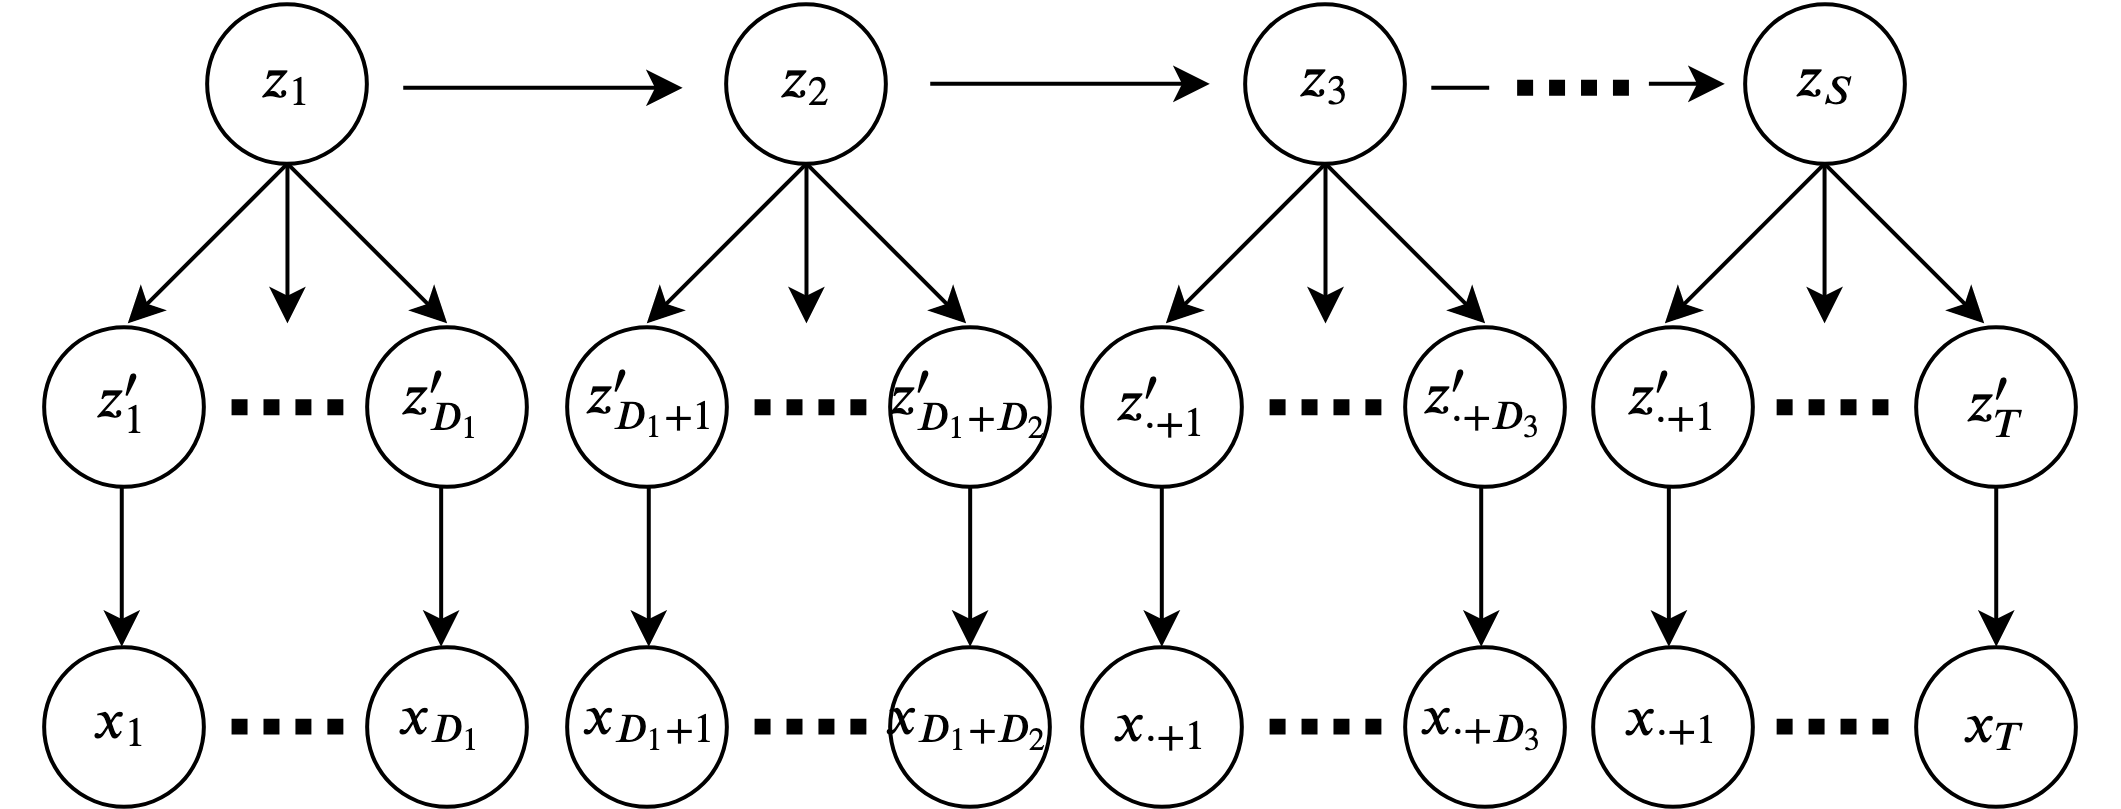
\includegraphics[scale=0.10]{images/hsmm2.png}
\caption{HSMM where super state transitions are Markovian, while emissions associated with each state follow some explicit duration distribution.}
\label{fig:hsmm}
\end{figure}

\subsection{Hierarchical Dirichlet Process HSMM (HDP-HSMM)}
We begin this section by reviewing the formulation of a hierarchical Dirichlet process HMM (HDP-HMM), which is a Bayesian non-parametric treatment of the classical HMM. A HDP-HMM$(\gamma, \alpha, H)$ model is a process governed by:
\begin{itemize}
  \item $\beta_k \coloneqq \beta_k'\cdot \prod_{i=1}^{k-1} (1-\beta_i')$ where $\beta_i' \overset{\text{i.i.d}}{\sim} Beta(1,\gamma)$
  \item $\pi_k \overset{\text{i.i.d}}{\sim} DP(H(\beta), \alpha)$ for $k = 1, \dots, \infty$ where $\beta = \{\beta_k\}_{k=1}^{\infty}$
  \item $z_t \sim \pi_{z_{t-1}}$
  \item $x_t \sim h(\theta_{z_t})$ where $\theta_{k} \sim H$ for $k = 1, \dots, \infty$
\end{itemize}
where $\gamma, \alpha > 0$ can be interpreted as concentration parameters and $H$ is the base distribution of the Dirichlet process. Note that $\{\beta_k\}_{k=1}^{\infty}$ is generated from a stick-breaking process with concentration parameter $\gamma$. These are then used in the generation of  transition distributions $\{\pi_k \}_{k=1}^{\infty}$ from a Dirichlet process with parameters $H$ and $\alpha$, where $H$ is defined on the $\{\beta_k\}_{k=1}^{\infty}$ partitions of the measurement set. For $t = 1, \dots, T$, each state $z_t$ is drawn from a respective $\pi_{z_{t-1}}$, and each observation is drawn from an observation distribution $h(\theta_{z_t})$ where $\theta_{k}$ is drawn from $H$. Observe that as $\alpha$ decreases, distributions $\{\pi_k\}_{s=1}^{\infty}$ tend to be more concentrated, and as $\gamma$ decreases, $\{\beta_k\}_{k=1}^{\infty}$ tends to zero and $\{h(\theta_{z_t})\}_{t=1}^{T}$ tends to be more concentrated as a result.

HDP-HSMM is an augmentation of the HDP-HMM to include duration distributions. Continuing from the notation above yields:
\begin{itemize}
  \item $\beta_k \coloneqq \beta_k'\cdot \prod_{i=1}^{k-1} (1-\beta_i')$ where $\beta_i' \overset{\text{i.i.d}}{\sim} Beta(1,\gamma)$
  \item $\pi_k \overset{\text{i.i.d}}{\sim} DP(H(\beta), \alpha)$ for $k = 1, \dots, \infty$ where $\beta = \{\beta_k\}_{k=1}^{\infty}$
  \item $z_s \sim \tilde{\pi}_{z_{s-1}}$
  \item $D_s \sim g(\omega_{z_s})$ where $\omega_k \sim G$ for $k = 1, \dots, \infty$
  \item $z'_{t_{s}:t'_{s}} = z_s$ where $t_{s} = \sum_{s' < s} D_s + 1$ and $t'_{s} = t_{s} + D_s - 1$
  \item $x_{t_{s}: t'_{s}} \overset{\text{i.i.d}}{\sim} h(\theta_{z'_t})$ where $\theta_{k} \sim H$ for $k = 1, \dots, \infty$
\end{itemize}

The main differences here are that we introduce a base distribution $G$ for drawing durations $D_s$ in a similar way that $H$ is defined in the HSMM setting which we use for drawing $\pi$. The duration distribution sequence of sub-states $z'_{t_{s}:t'_{s}}$ is set to the corresponding super-state $z_{s}$ where $t_{s}$ is the starting index for the sub-state sequence corresponding to super-state $z_s$, and $t'_{s}$ is the end index for the sub-state sequence corresponding to super-state $z_s$. The observation sequence is then drawn from the sub-state sequence using $H$. Note that $z_s$ is drawn from $\tilde{pi}_{k} \coloneqq \frac{\pi_{k,j}}{1-\pi_{k,k}}(1 - \delta_{k,j})$, which normalizes $\pi_k$ to prevent self-transitions in the super-state sequence $z_s$. Figure ~\ref{fig:hdphsmm} extends the previous HSMM diagram to illustrate the connections between the HDP component of the model, and the HSMM.

\begin{figure}[H]
\centering
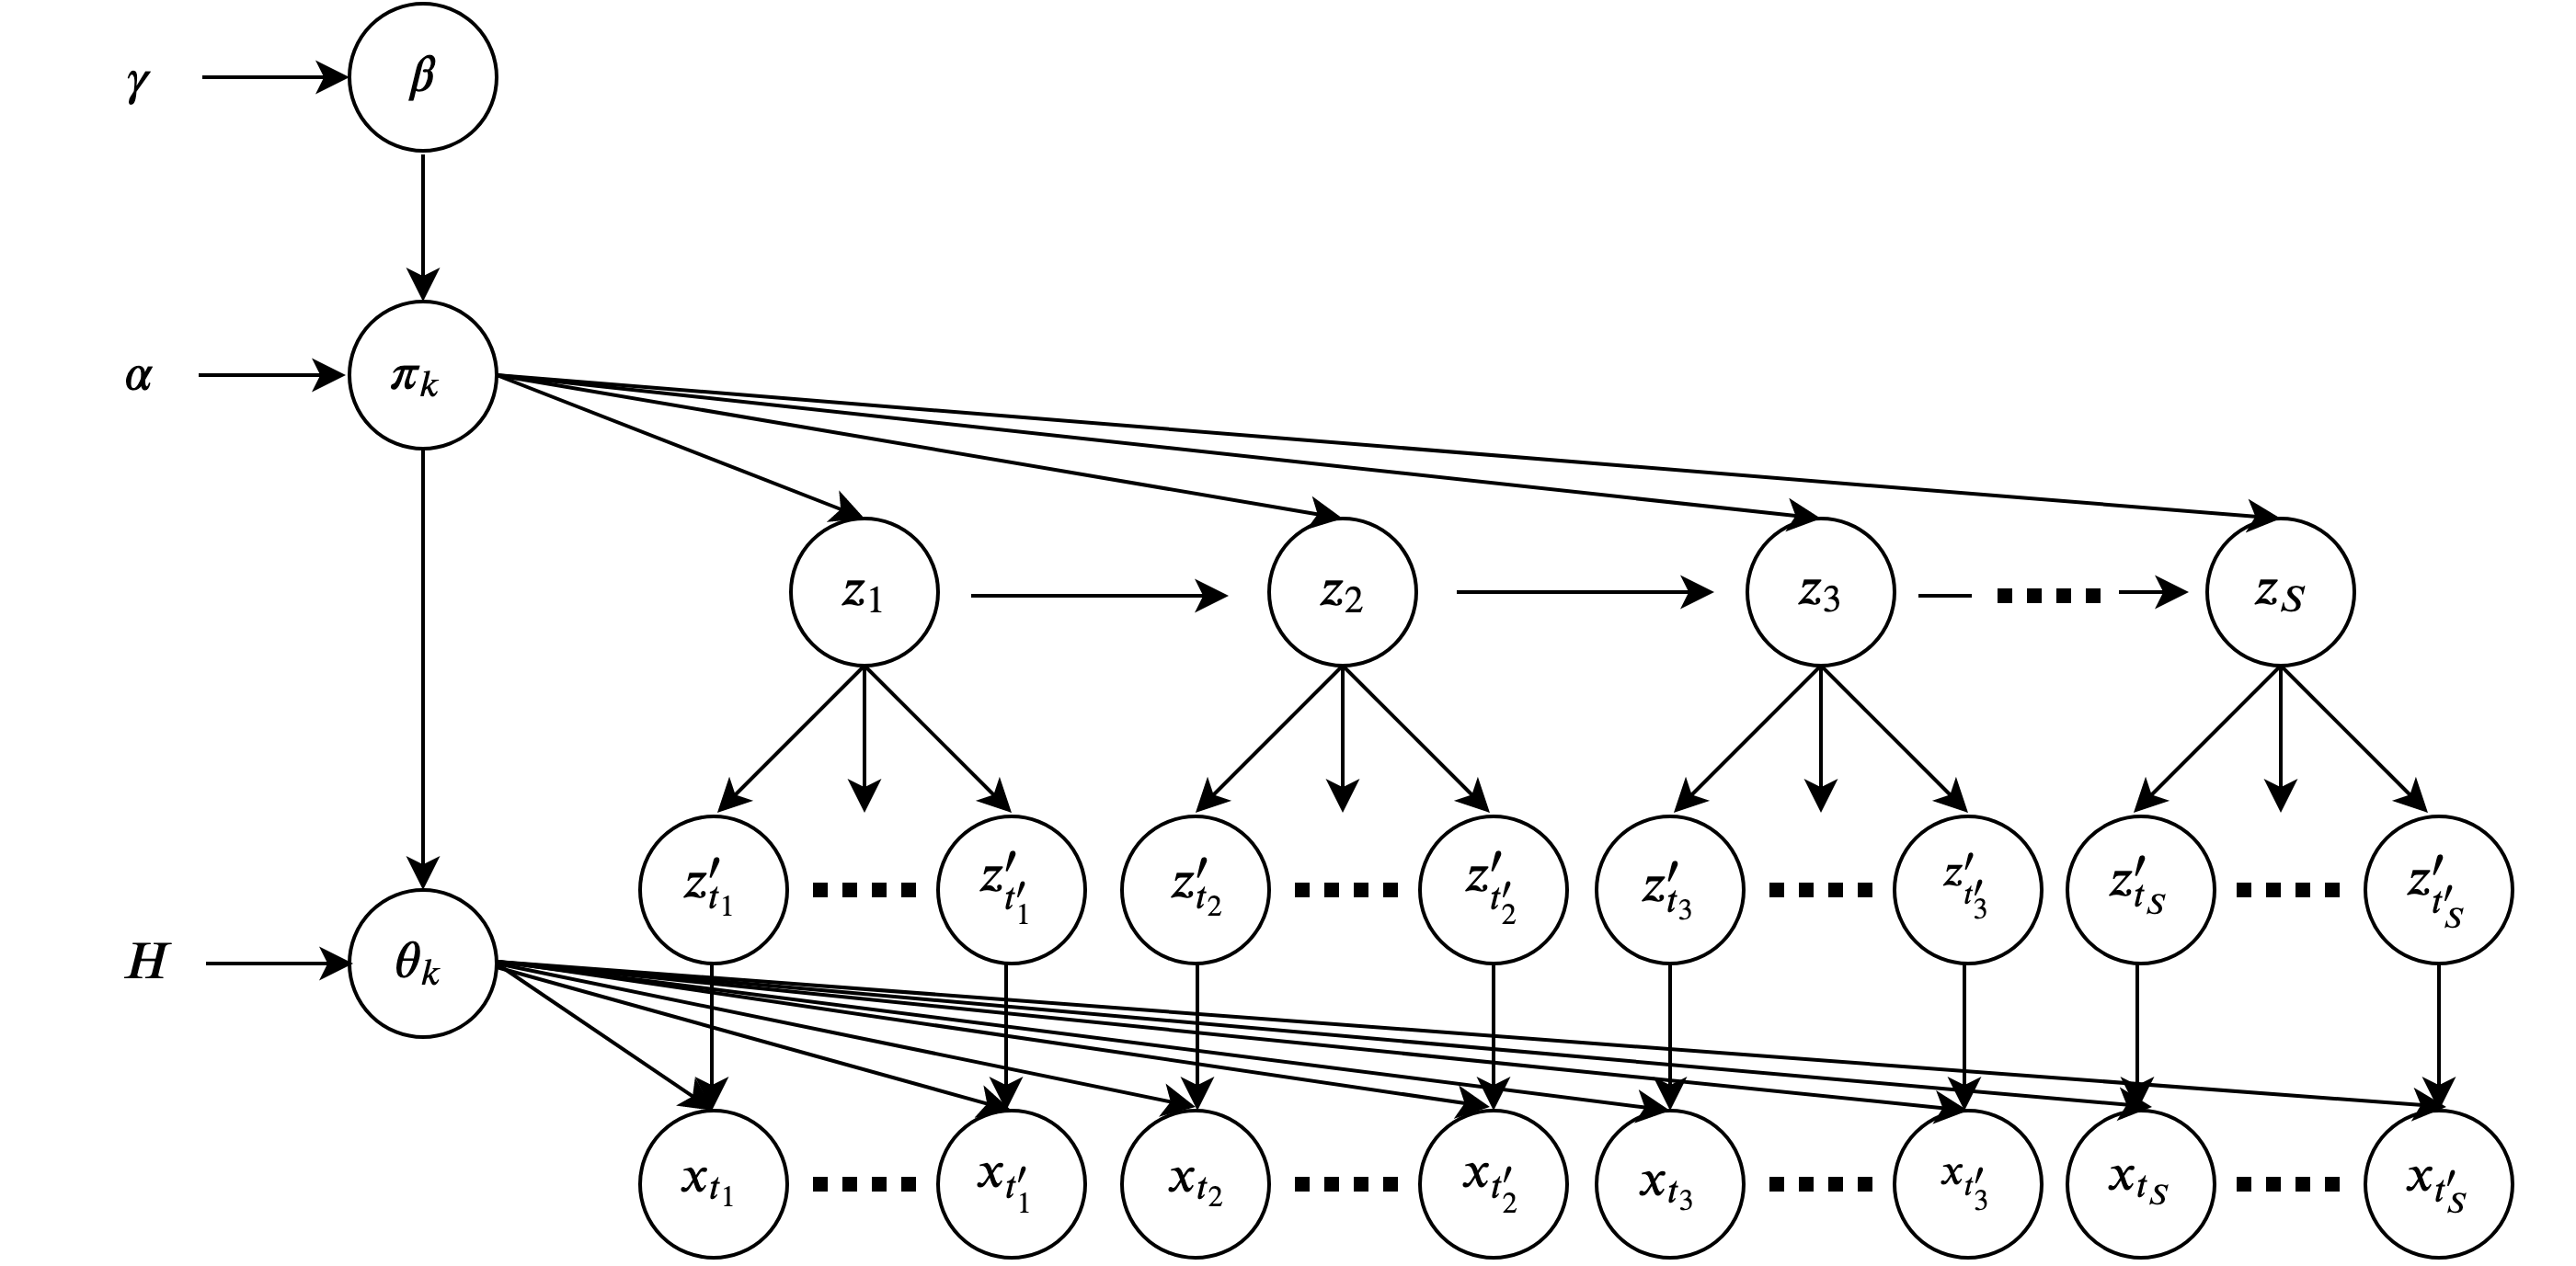
\includegraphics[scale=0.10]{images/hdphsmm.png}
\caption{HDP-HSMM incorporates a HDP component into a HSMM}
\label{fig:hdphsmm}
\end{figure}

\section{Simulating Agent States and Observations}

To generate the agent pathways and observations, we varied the following grid settings and motion model assumptions:

\begin{enumerate}
	\item \textbf{Grid Size}: We generated pathways on 5$\times$5 grids, so each grid has 25 hidden states.
	\item \textbf{Obstacles}: Obstacles are placed in each grid by making certain states impossible to visit -- this is analogous to a robot encountering physical boundaries, like walls or other objects.
	\item \textbf{Markov Property}: We simulated different settings for the transition matrix between states, with one setting violating the Markov assumption. Further details of these settings in Section 2.2.
\end{enumerate}

\subsection{GridWorld Setup}

We simulated pathways on the following three grids. Each square in the grid either has a number representing its true observation, or is colored black, indicating an obstacle.

\newcommand{\addmapa}{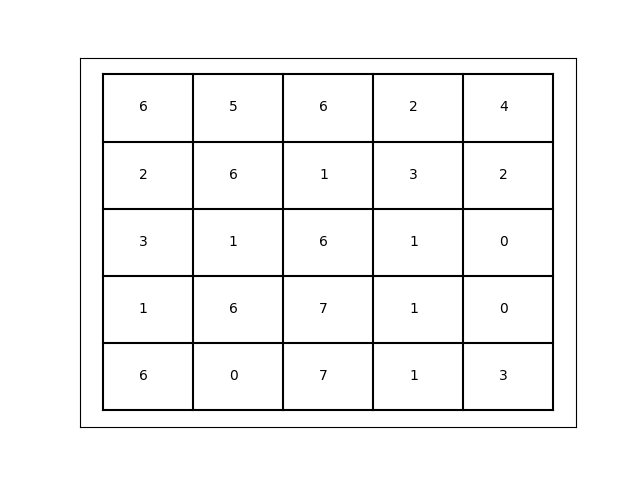
\includegraphics[width=10em]{data/Model1/5x5;4;free.png}}
\newcommand{\addmapb}{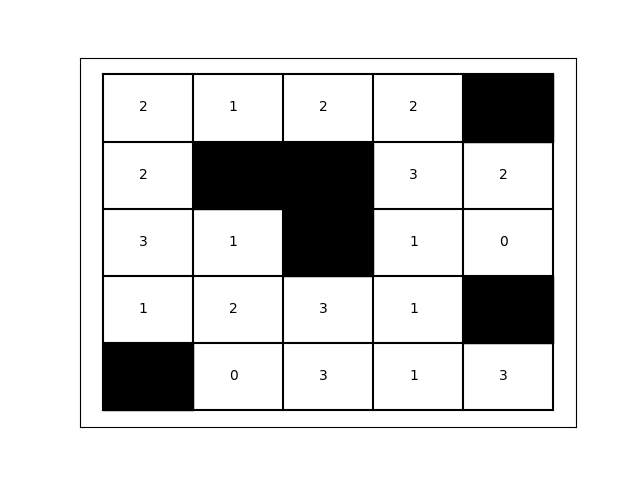
\includegraphics[width=10em]{data/Model2/5x5;4;6box.png}}
\newcommand{\addmapc}{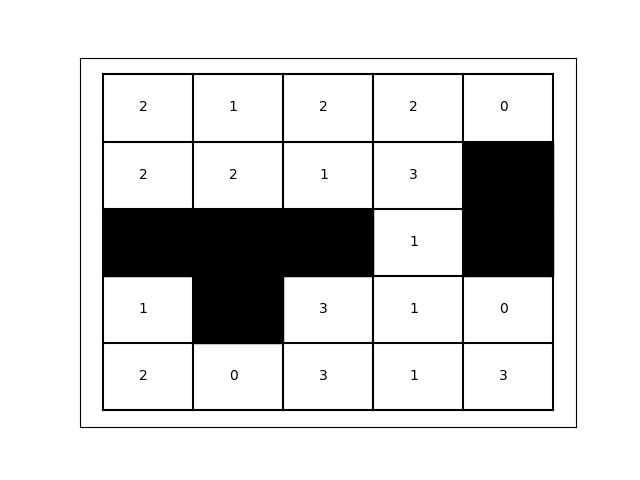
\includegraphics[width=10em]{data/Model3/5x5;4;6sep.png}}
\newcolumntype{C}{>{\centering\arraybackslash}m{10em}}
\begin{table}[H]
\sffamily
\centering
\begin{tabular}{l*4{C}@{}}
& \addmapa & \addmapb & \addmapc \\
\end{tabular}
\caption{GridWorld Maps}
\end{table}

\subsection{Motion Settings}

As stated above, the path for each grid was simulated using three different settings for the transitions between states.

\begin{enumerate}
	\item \textbf{Purely Random}: The agent transitions from state to state with a uniform transition probability over all of the states (including its current state) -- each step is essentially randomly generated with replacement from the set of valid states. This setting satisfies the Markov property.
	\item \textbf{Traditional Markov}: The state sequences are generated using a fixed transition matrix -- the probability of transitioning from a given state to the next state is constant as the sequence is generated, and each step is independent of past states conditional on the present state. This setting satisfies the Markov property.
	\item \textbf{Sticky Transitions}: The HDP-HSMM specializes in inferring observations when the underlying motion is presumed to be "sticky". Specifically, a sticky process is one where transition probabilities correspond to an agent's elapsed duration in the same state. In our implementation, the probability of staying in the same state decreases geometrically with the duration, and resets upon entering a new state.
 \end{enumerate}

To generate the "true" transition matrix from which the robot path would be simulated, we first generated a matrix where the probability of staying in the same state was $0.2$. This probability was constant in the Traditional Markov setting, while it decreased geometrically in the Sticky Transitions setting. We then perturbed this probability using a randomly generated value between $-0.1$ and $0.1$. To fill out the transition matrix, we then evenly distributed the remaining probability among valid adjacent states.

\subsection{Observation Settings}

To compare the original HMM and HDP-HSMM, we simulate observations that are continuous measurements. Each state is assigned a true mean $\mu$, while the standard deviation is identical and fixed at $\sigma = 0.5$. There were eight possible true values of $\mu$, so some of the states had the same observation mean. The agent observes a Gaussian sample given the mean of the state.

To generate our data, for each of the 9 settings (3 grids x 3 transition settings), we simulate 10 state sequences of length 200. Then, observations from these state sequences are generated using the emission distributions, where the "true" observation for each state was randomly assigned. These generated observation sequences were used as the inputs for our HMM and HDP-HSMM.

\section{Results}

To measure the accuracy of the HMM and HDP-HSMM methods, we measured the misclassification rate between the state sequences estimated by each method from the observation sequences, and the true state sequences from which the observations were generated. Our results below are the median misclassification rate across our 10 generated sequences using each method.

\begin{table}[H]	
	\centering
	\subfloat[HMM Results]{
		\begin{tabular}{|l|l|l|l|}
		\hline
		& Map 1 & Map 2 & Map 3 \\
		\hline
		Random	& 0.908 & 0.908 & 0.908  \\
		\hline
		Markov & 0.483 & 0.435 & 0.440 \\
		\hline
		Sticky & 0.460 & 0.475& 0.503 \\
		\hline
		\end{tabular}
	}
	\subfloat[HDP-HSMM Results]{
	\begin{tabular}{|l|l|l|l|}
		\hline
		& Map 1 & Map 2 & Map 3 \\
		\hline
		Random	& 0.908 & NA &  NA \\
		\hline
		Markov & 0.768 & 0.758 & 0.765 \\
		\hline
		Sticky & 0.790 & 0.788 & 0.785 \\
		\hline
		\end{tabular}
	}
	%\caption{HDP-HSMM Results}
	% \caption{HMM Results}
	
\end{table}


\section{Discussion}

\subsection{Markov Property and Obstacles in HMM}

The results of applying the Baum-Welch and Viterbi algorithm to our simulated sequences largely confirm that relaxing the Markov assumption does not lead to significantly worse results. The misclassification rate in the sticky transition setting was no more than 6 percentage points worse than the Markovian setting. This small reduction in accuracy is acceptable, as it allows the application of the method to many more data sets -- real data often violates the Markov assumption.

An interesting result was the effect of the number and placement of obstacles on the map. In the Markovian setting, the misclassification rate for the two maps with obstacles, Maps 2 and 3, were lower than the rate for Map 1, with no obstacles. By reducing the total number of valid states and the number of possible pathways, obstacles actually make it easier to estimate the hidden state sequence of the agent. This pattern was reversed in the sticky transition setting, though we do not have a strong intuitive explanation for this observation.

We also discovered observation generation settings under which the method performed very poorly. If we set the number of possible true $\mu$ values to be small -- so many states shared the same mean -- the misclassification rate was sharply higher. The more possibilities there were, the better the algorithm performed. This made sense to us, as the method would have a hard time determining which state a certain observation came from if many states had a similarly high likelihood under the emission distribution.

\subsection{Comparing HMM and HDP-HSMM}

Compared to the HMM, the HDP-HSMM performs noticably poorer across the different grid and motion settings, which is somewhat unexpected. There are a number of possible explanations for why this may have occurred based on our implementation:

\begin{itemize}
  \item \textbf{Inferring the number of states:} A particular challenge common across non-parametric methods is that the HDP-HSMM must correctly infer the true number of states without user-supplied prior information. Our implementation uses 25 states where each state had a true mean that was one of eight possible distinct values -- this can result in many states being easily mistaken by the HDP-HSMM to be the same state. We illustrate this phenomenon in Table~\ref{table:meaninfer} below, where the estimated state means (blue) are plotted against the true state means (green). Here, we provide some assistance to the HDP-HSMM algorithm by putting a threshold on the maximum number of total states. HDP-HSMM infers a mean for each Gaussian but only a subset of these are used (red) for inference, which tend to congregate towards regions where the means are relatively large with respect to the fixed $\sigma$. It follows that states where the true means are similar and relatively small with respect to the fixed $\sigma$ tend to be overlooked as distinct states, which then leads to higher misclassification error.
  \item \textbf{Strength of non-Markovity:} Our simulations begin by initializing a probability level ($0.2$) for the agent to stay in the same state at any given timestep, which then defines the rest of the transition matrix. Using this level in the sticky motion model tends to only produce weak non-Markovity since the probability of transitioning to a new state is relatively high, and any stickiness to the same state will be ephemeral compared to settings where the probability level is larger as a result of the properties of the geometric distribution. We illustrate this phenomenon in Table~\ref{table:stateinfer} where the sticky motion model is very similar to our Markovian motion.
  \item \textbf{Convergence:} There is some concern about whether HDP-HSMM converged sufficiently in our experiments. Tests with longer sequences and more sequences did not yield significantly different results, but it is not clear what scale is appropriate given the problem space. HDP-HSMM did not converge for the random motion models in Maps 2 and 3, which suggests that having one universal setting for sequence length and number of sequences for all problems may not be appropriate.
\end{itemize}

\newcommand{\addrandommeana}{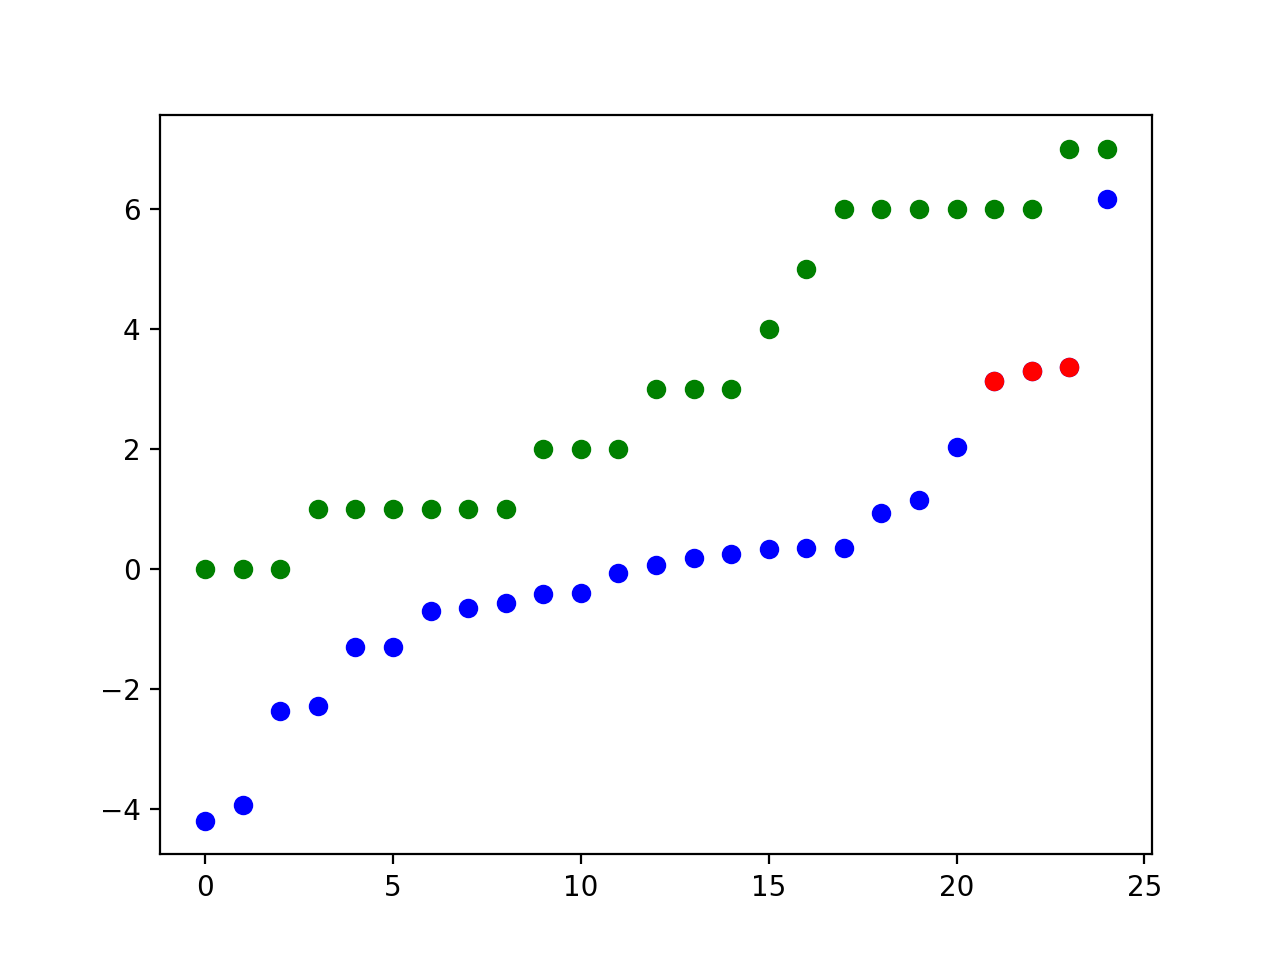
\includegraphics[width=10em]{images/hdphsmm/random-m1-means.png}}
\newcommand{\addmarkovmeana}{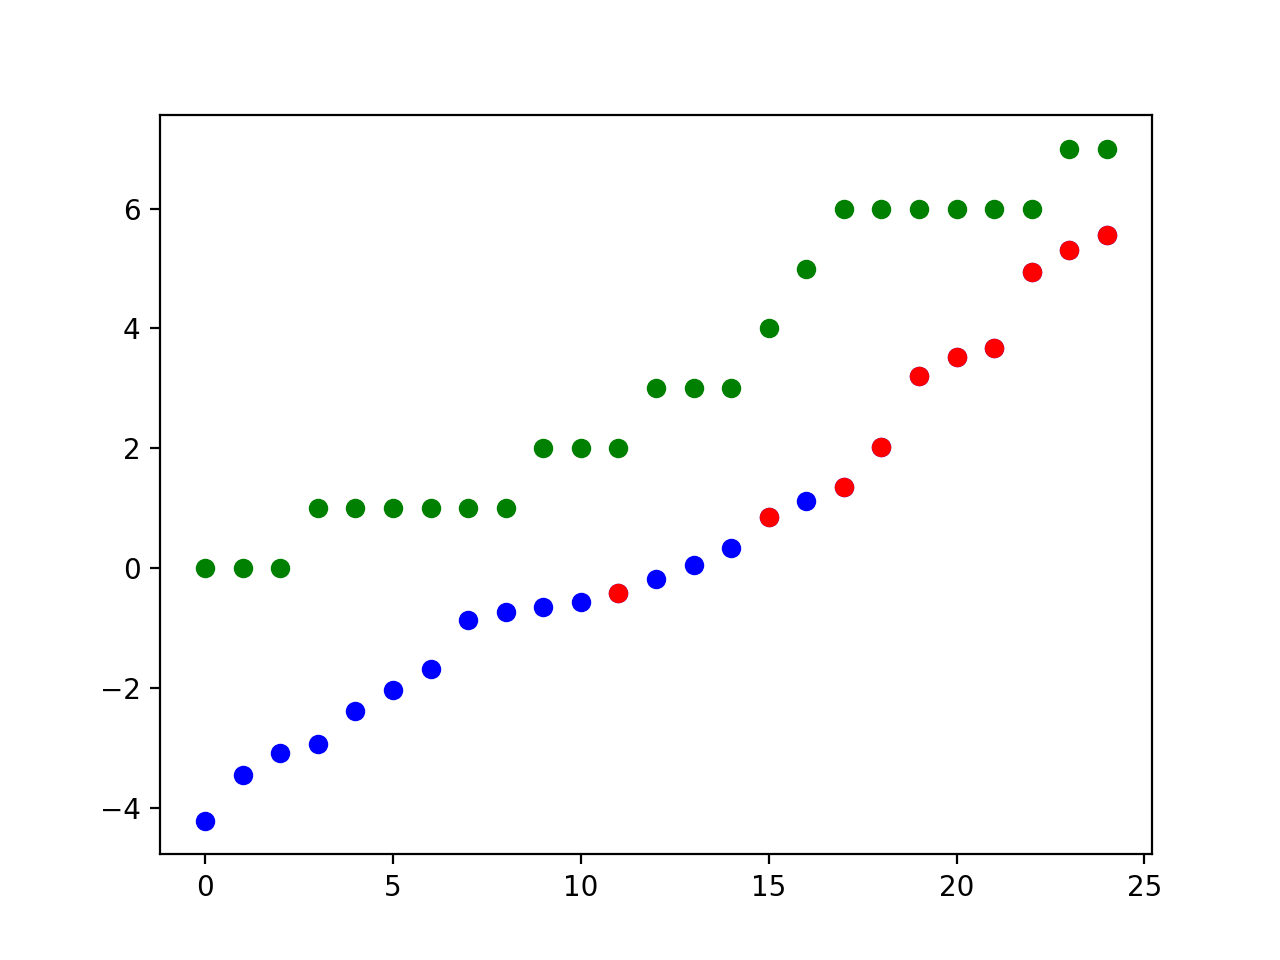
\includegraphics[width=10em]{images/hdphsmm/markov-m1-means.png}}
\newcommand{\addcorrmeana}{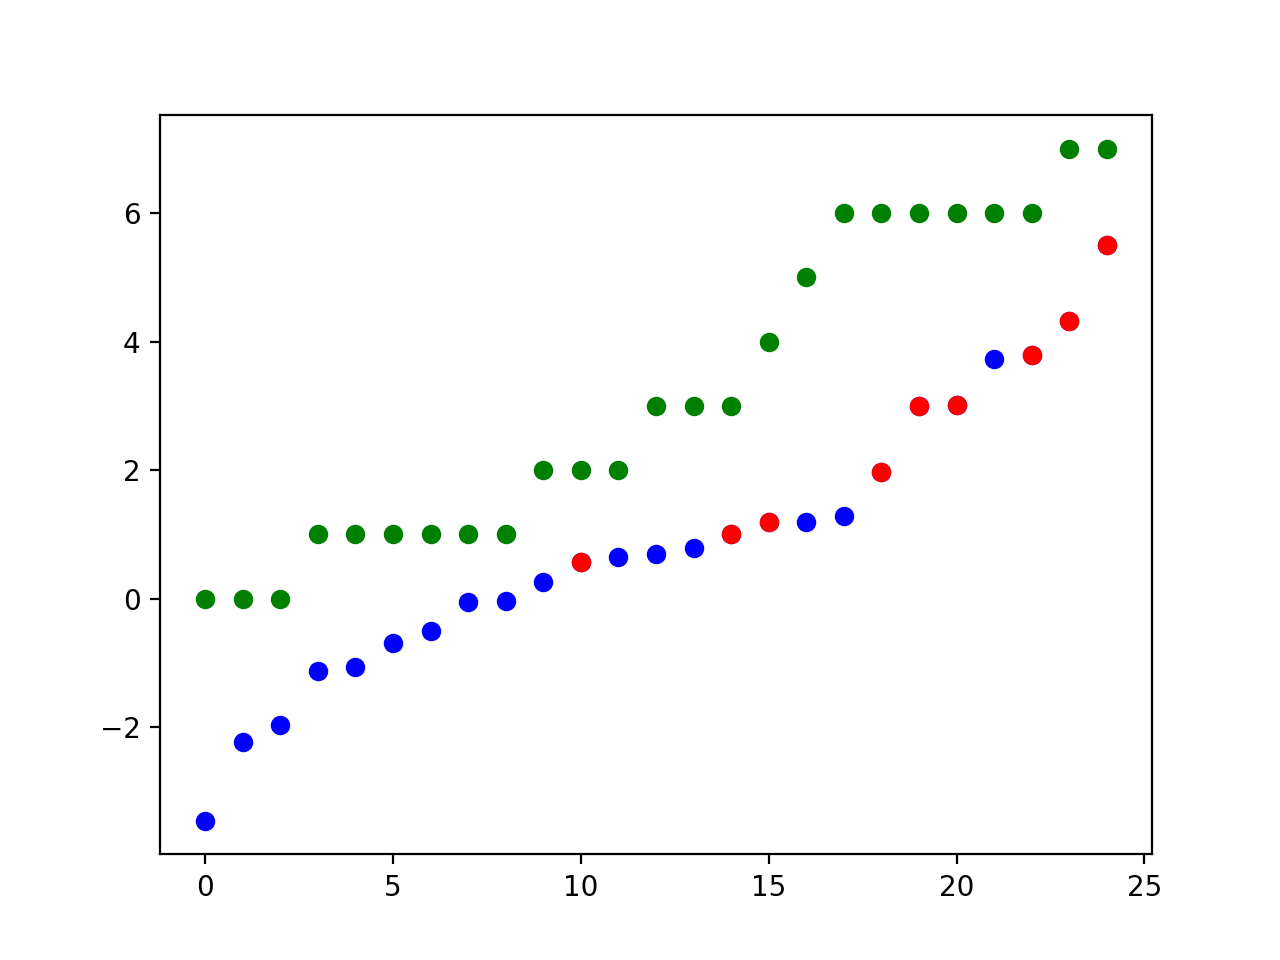
\includegraphics[width=10em]{images/hdphsmm/corr-m1-means.png}}
\begin{table}[H]
\sffamily
\centering
\begin{tabular}{l*4{C}@{}}
& \addrandommeana & \addmarkovmeana & \addcorrmeana \\
\end{tabular}
\caption{Estimated means and true means for different motions (random, Markov and sticky) through Map 1}
\label{table:meaninfer}
\end{table}

\newcommand{\addrandomseqa}{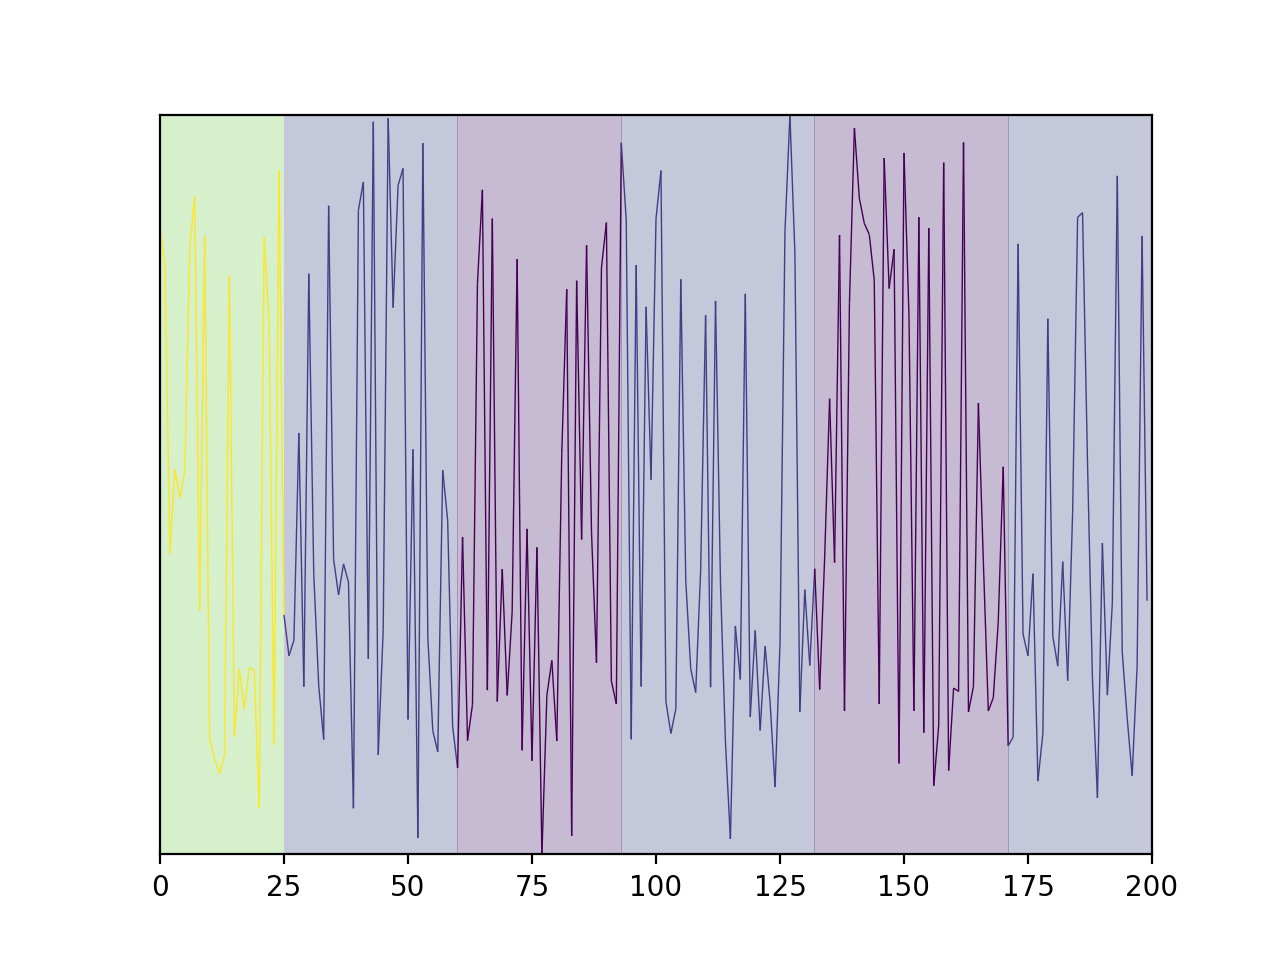
\includegraphics[width=10em]{images/hdphsmm/random-m1-seq.png}}
\newcommand{\addmarkovseqa}{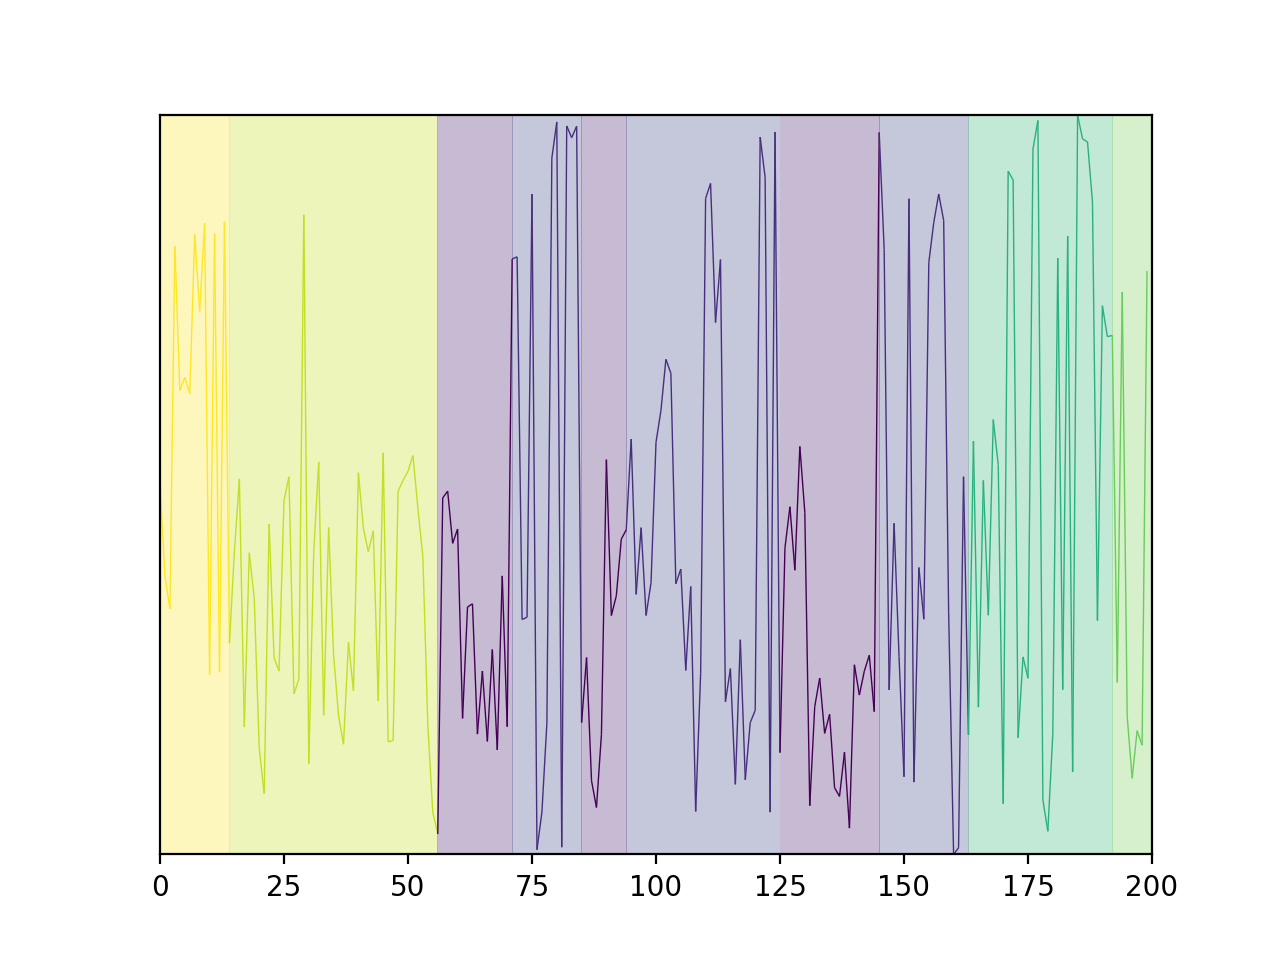
\includegraphics[width=10em]{images/hdphsmm/markov-m1-seq.png}}
\newcommand{\addcorrseqa}{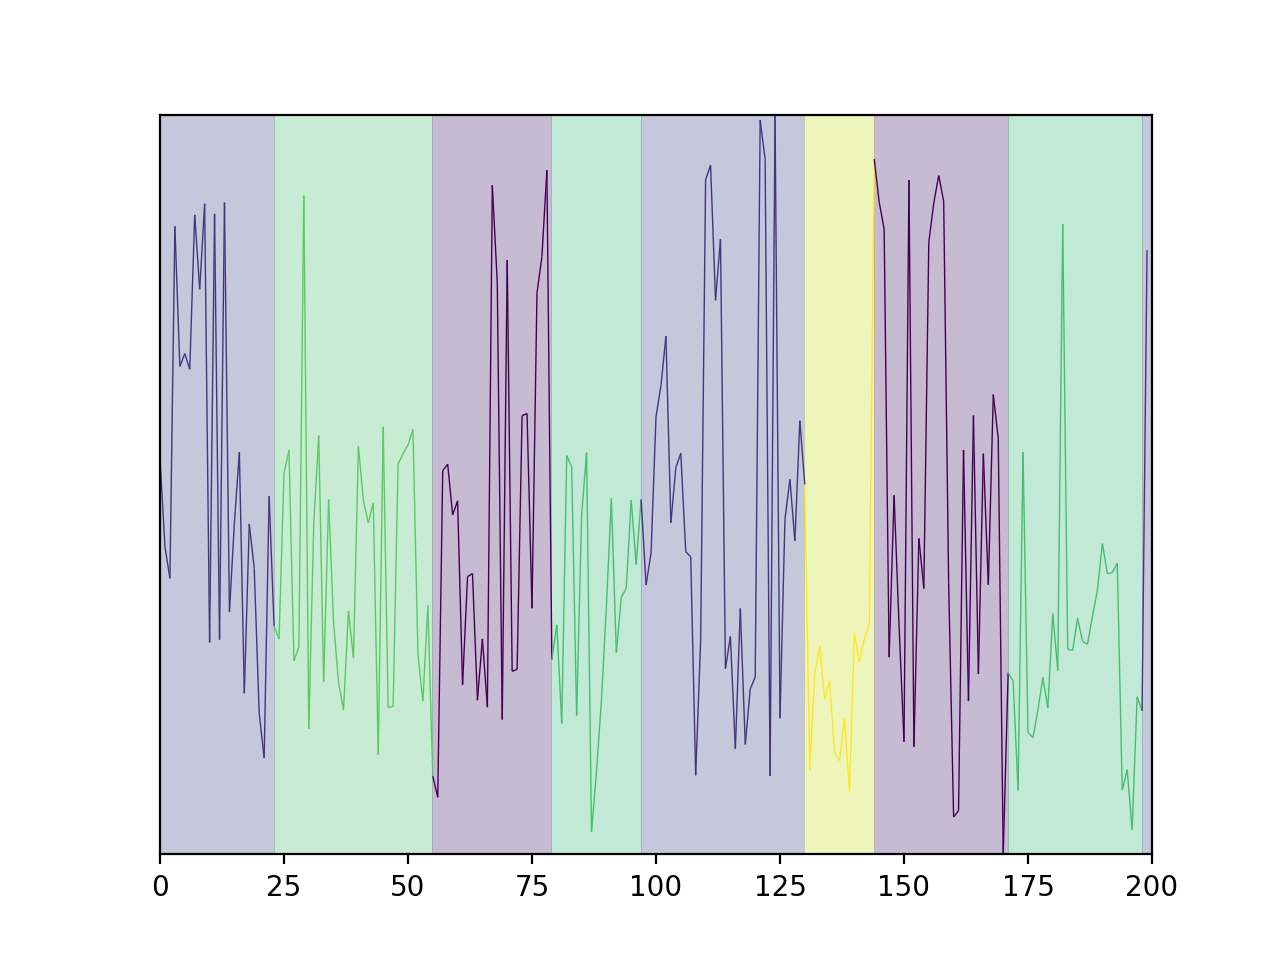
\includegraphics[width=10em]{images/hdphsmm/corr-m1-seq.png}}
\begin{table}[H]
\sffamily
\centering
\begin{tabular}{l*4{C}@{}}
& \addrandomseqa & \addmarkovseqa & \addcorrseqa \\
\end{tabular}
\caption{Observation sequences mapped to inferred states for different motions (random, Markov and sticky) through Map 1}
\label{table:stateinfer}
\end{table}

\section{Conclusions and Future Work}

We drew two primary conclusions from our study:

\begin{itemize}
	\item \textbf{HMM Performance in Non-Markov Settings}: The classic HMM method produced reasonable results even when applied to data that violates the Markov assumption. The loss in accuracy is acceptable for the ability to apply the method to non-Markovian data.
	\item \textbf{Accuracy of HMM vs. HDP-HSMM}: In our test settings, the HMM method had a much lower misclassification rate than the HDP-HSMM method. This result likely came about because we had knowledge of how the data was generated. We were able to set up the HMM with a well-informed prior, while the HDP-HSMM method struggled to infer the correct number of states. We likely would have seen different results if we did not have any information with which to set up a strong prior for the HMM method.
\end{itemize}

Based on these conclusions, there are several avenues to extend our work:

\begin{itemize}
	\item For reasons of time, we limited our study to 2,000 simulated observations, with one random seed setting. There is a great deal of scope to expand our experiments through generating more data, including using different random generator seeds, different grid sizes and obstacle placements, and adjusting the transition and emission distributions.
	\item We could test the accuracy of the HMM under less-informative priors. From our testing, increasing the closeness of the prior to the true distributions had a strong effect on accuracy, so it could be interesting to empirically test the importance of having good prior distributions.
	\item We could strengthen the non-Markovity and make the true means of the states more distinct, to see how the HDP-HSMM performs in that setting. Our simulated data in this paper was designed to test the Markov assumption for HMMs, while the HDP-HSMM was proposed to deal with a different set of data problems.
\end{itemize}

\newpage

\section*{References}
\medskip

\small

[1] Johnson, M.J.\ \& Willsky, A.S.\ (2013) Bayesian Nonparametric Hidden Semi-Markov Models, {\it Journal of Machine Learning Research 14 (2013)},
pp.\ 673--701. Cambridge, MA: MIT Press.

\end{document}